\documentclass{standalone}
\usepackage{tikz}
\usetikzlibrary{patterns, positioning}
\usepackage[sfdefault]{ClearSans} %% option 'sfdefault' activates Clear Sans as the default text font
\usepackage[T1]{fontenc}

\begin{document}
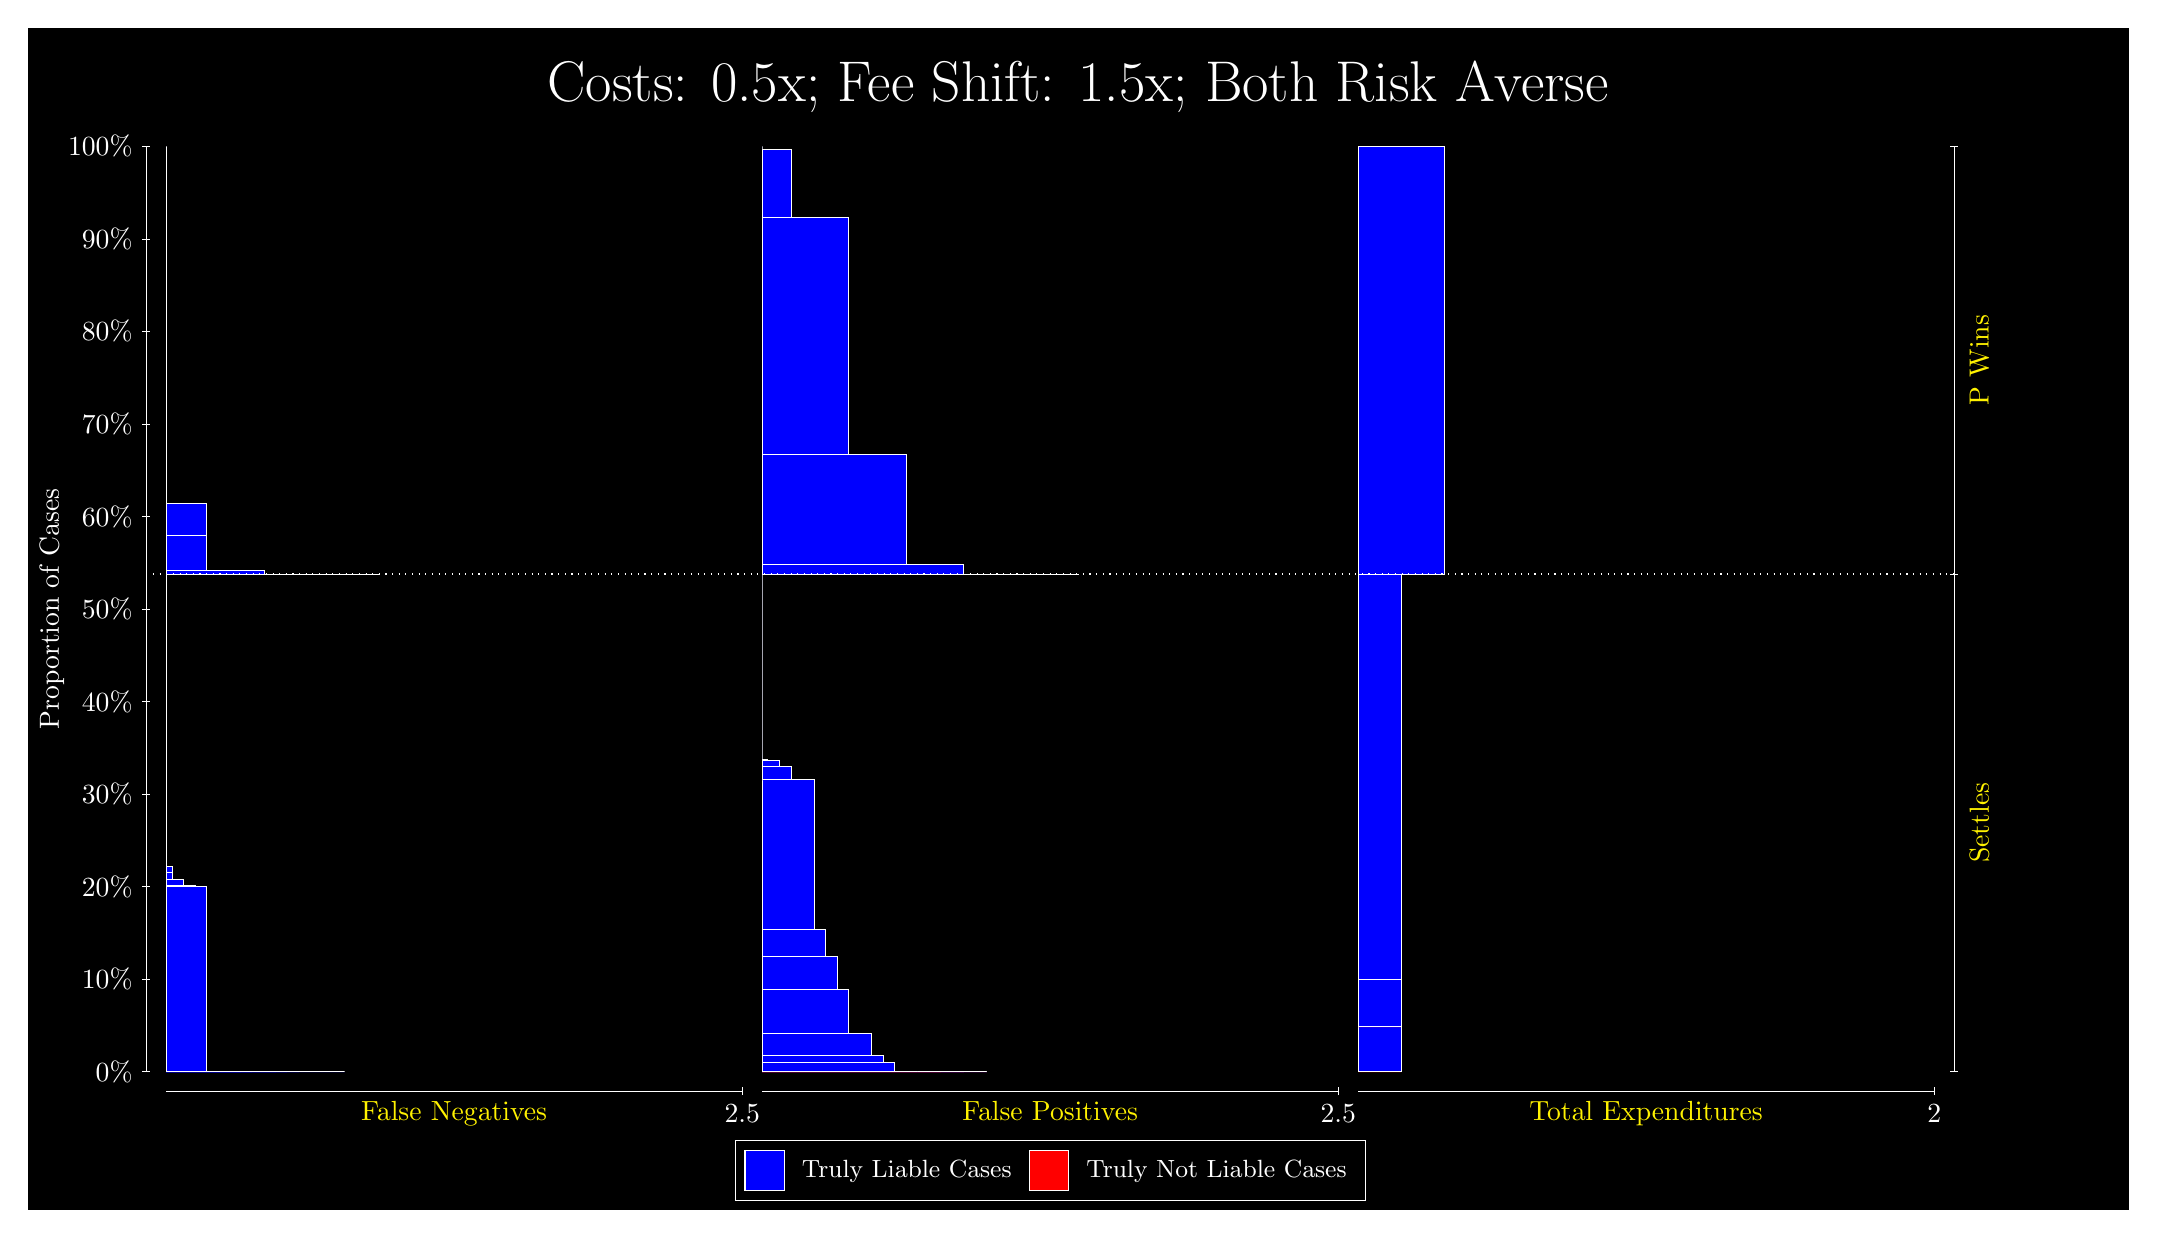
\begin{tikzpicture}
\draw[fill=black] (0,0) rectangle (26.667,15);
\draw[text=white] (0,13.5) rectangle (26.667,15) node[midway] {\huge Costs: 0.5x; Fee Shift: 1.5x; Both Risk Averse};
\draw[white, very thin] (1.5,1.75) -- (1.5,13.5);
\node[rotate=90, text=white, anchor=center] at (0.3, 7.625) {Proportion of Cases};
\draw[white, very thin] (1.45,1.75) -- (1.55,1.75);
\node[text=white, anchor=east] at (1.45, 1.75) {0\%};
\draw[white, very thin] (1.45,2.925) -- (1.55,2.925);
\node[text=white, anchor=east] at (1.45, 2.925) {10\%};
\draw[white, very thin] (1.45,4.1) -- (1.55,4.1);
\node[text=white, anchor=east] at (1.45, 4.1) {20\%};
\draw[white, very thin] (1.45,5.275) -- (1.55,5.275);
\node[text=white, anchor=east] at (1.45, 5.275) {30\%};
\draw[white, very thin] (1.45,6.45) -- (1.55,6.45);
\node[text=white, anchor=east] at (1.45, 6.45) {40\%};
\draw[white, very thin] (1.45,7.625) -- (1.55,7.625);
\node[text=white, anchor=east] at (1.45, 7.625) {50\%};
\draw[white, very thin] (1.45,8.8) -- (1.55,8.8);
\node[text=white, anchor=east] at (1.45, 8.8) {60\%};
\draw[white, very thin] (1.45,9.975) -- (1.55,9.975);
\node[text=white, anchor=east] at (1.45, 9.975) {70\%};
\draw[white, very thin] (1.45,11.15) -- (1.55,11.15);
\node[text=white, anchor=east] at (1.45, 11.15) {80\%};
\draw[white, very thin] (1.45,12.325) -- (1.55,12.325);
\node[text=white, anchor=east] at (1.45, 12.325) {90\%};
\draw[white, very thin] (1.45,13.5) -- (1.55,13.5);
\node[text=white, anchor=east] at (1.45, 13.5) {100\%};

\draw[white, very thin] (24.457,1.75) -- (24.457,13.5);
\draw[white, very thin] (24.407,1.75) -- (24.507,1.75);
\node[anchor=west] at (24.407, 1.75) {};
\draw[white, very thin] (24.407,8.0689) -- (24.507,8.0689);
\node[anchor=west] at (24.407, 8.0689) {};
\draw[white, very thin] (24.407,13.5) -- (24.507,13.5);
\node[anchor=west] at (24.407, 13.5) {};

\draw[white, very thin, fill=blue] (1.75,1.75) rectangle (4.0188,1.75);
\draw[white, very thin, fill=blue] (1.75,1.75) rectangle (3.4333,1.75);
\draw[white, very thin, fill=blue] (1.75,1.75) rectangle (3.287,1.75);
\draw[white, very thin, fill=blue] (1.75,1.75) rectangle (3.1406,1.75);
\draw[white, very thin, fill=blue] (1.75,1.75) rectangle (2.8478,1.75);
\draw[white, very thin, fill=blue] (1.75,1.75) rectangle (2.7015,1.7501);
\draw[white, very thin, fill=blue] (1.75,1.7501) rectangle (2.5551,1.7508);
\draw[white, very thin, fill=blue] (1.75,1.7508) rectangle (2.5551,1.7517);
\draw[white, very thin, fill=blue] (1.75,1.7517) rectangle (2.4087,1.7517);
\draw[white, very thin, fill=blue] (1.75,1.7517) rectangle (2.2623,4.097);
\draw[white, very thin, fill=blue] (1.75,4.097) rectangle (2.1159,4.1123);
\draw[white, very thin, fill=blue] (1.75,4.1123) rectangle (1.9696,4.1906);
\draw[white, very thin, fill=blue] (1.75,4.1906) rectangle (1.8232,4.283);
\draw[white, very thin, fill=blue] (1.75,4.283) rectangle (1.8232,4.3615);
\draw[white, very thin, fill=red] (1.75,4.3615) rectangle (1.75,4.3615);
\draw[white, very thin, fill=blue] (1.75,4.3615) rectangle (1.75,8.0689);
\draw[white, very thin, fill=blue] (1.75,8.0689) rectangle (4.458,8.0689);
\draw[white, very thin, fill=blue] (1.75,8.0689) rectangle (3.7261,8.069);
\draw[white, very thin, fill=blue] (1.75,8.069) rectangle (2.9942,8.1122);
\draw[white, very thin, fill=blue] (1.75,8.1122) rectangle (2.2623,8.5565);
\draw[white, very thin, fill=blue] (1.75,8.5565) rectangle (2.2623,8.9671);
\draw[white, very thin, fill=red] (1.75,8.9671) rectangle (1.75,8.9671);
\draw[white, very thin, fill=blue] (1.75,8.9671) rectangle (1.75,13.5);
\draw[white, very thin, fill=red] (9.3189,1.75) rectangle (12.173,1.75);
\draw[white, very thin, fill=blue] (9.3189,1.75) rectangle (12.173,1.75);
\draw[white, very thin, fill=red] (9.3189,1.75) rectangle (11.88,1.75);
\draw[white, very thin, fill=blue] (9.3189,1.75) rectangle (11.88,1.75);
\draw[white, very thin, fill=red] (9.3189,1.75) rectangle (11.588,1.75);
\draw[white, very thin, fill=blue] (9.3189,1.75) rectangle (11.588,1.7509);
\draw[white, very thin, fill=blue] (9.3189,1.7509) rectangle (11.441,1.7525);
\draw[white, very thin, fill=red] (9.3189,1.7525) rectangle (11.295,1.7525);
\draw[white, very thin, fill=blue] (9.3189,1.7525) rectangle (11.295,1.7525);
\draw[white, very thin, fill=blue] (9.3189,1.7525) rectangle (11.149,1.7533);
\draw[white, very thin, fill=red] (9.3189,1.7533) rectangle (11.002,1.7533);
\draw[white, very thin, fill=blue] (9.3189,1.7533) rectangle (11.002,1.8639);
\draw[white, very thin, fill=blue] (9.3189,1.8639) rectangle (10.856,1.957);
\draw[white, very thin, fill=blue] (9.3189,1.957) rectangle (10.709,2.2365);
\draw[white, very thin, fill=blue] (9.3189,2.2365) rectangle (10.563,2.2367);
\draw[white, very thin, fill=red] (9.3189,2.2367) rectangle (10.417,2.2367);
\draw[white, very thin, fill=blue] (9.3189,2.2367) rectangle (10.417,2.7918);
\draw[white, very thin, fill=blue] (9.3189,2.7918) rectangle (10.27,3.2075);
\draw[white, very thin, fill=blue] (9.3189,3.2075) rectangle (10.124,3.5597);
\draw[white, very thin, fill=blue] (9.3189,3.5597) rectangle (9.9776,5.4572);
\draw[white, very thin, fill=blue] (9.3189,5.4572) rectangle (9.8312,5.4573);
\draw[white, very thin, fill=blue] (9.3189,5.4573) rectangle (9.6848,5.6283);
\draw[white, very thin, fill=blue] (9.3189,5.6283) rectangle (9.5384,5.7066);
\draw[white, very thin, fill=blue] (9.3189,5.7066) rectangle (9.3921,5.7219);
\draw[white, very thin, fill=blue] (9.3189,5.7219) rectangle (9.3189,8.0689);
\draw[white, very thin, fill=red] (9.3189,8.0689) rectangle (13.344,8.0689);
\draw[white, very thin, fill=blue] (9.3189,8.0689) rectangle (13.344,8.0689);
\draw[white, very thin, fill=red] (9.3189,8.0689) rectangle (12.612,8.0689);
\draw[white, very thin, fill=blue] (9.3189,8.0689) rectangle (12.612,8.0707);
\draw[white, very thin, fill=red] (9.3189,8.0707) rectangle (11.88,8.0707);
\draw[white, very thin, fill=blue] (9.3189,8.0707) rectangle (11.88,8.198);
\draw[white, very thin, fill=red] (9.3189,8.198) rectangle (11.149,8.198);
\draw[white, very thin, fill=blue] (9.3189,8.198) rectangle (11.149,9.5932);
\draw[white, very thin, fill=red] (9.3189,9.5932) rectangle (10.417,9.5932);
\draw[white, very thin, fill=blue] (9.3189,9.5932) rectangle (10.417,12.602);
\draw[white, very thin, fill=blue] (9.3189,12.602) rectangle (9.6848,13.457);
\draw[white, very thin, fill=blue] (9.3189,13.457) rectangle (9.3189,13.5);
\draw[white, very thin, fill=red] (16.888,1.75) rectangle (17.437,1.75);
\draw[white, very thin, fill=blue] (16.888,1.75) rectangle (17.437,2.3198);
\draw[white, very thin, fill=red] (16.888,2.3198) rectangle (17.437,2.3198);
\draw[white, very thin, fill=blue] (16.888,2.3198) rectangle (17.437,2.9245);
\draw[white, very thin, fill=red] (16.888,2.9245) rectangle (17.437,2.9245);
\draw[white, very thin, fill=blue] (16.888,2.9245) rectangle (17.437,8.0689);
\draw[white, very thin, fill=red] (16.888,8.0689) rectangle (17.986,8.0689);
\draw[white, very thin, fill=blue] (16.888,8.0689) rectangle (17.986,13.5);
\draw[white, dotted] (1.5,8.0689) -- (24.457,8.0689);
\draw[white, very thin] (1.75,1.5) -- (9.0689,1.5);
\node[text=yellow, anchor=north] at (5.4094, 1.5) {False Negatives};
\draw[white, very thin] (9.0689,1.45) -- (9.0689,1.55);
\node[text=white, anchor=north] at (9.0689, 1.45) {2.5};

\draw[white, very thin] (9.3189,1.5) -- (16.638,1.5);
\node[text=yellow, anchor=north] at (12.978, 1.5) {False Positives};
\draw[white, very thin] (16.638,1.45) -- (16.638,1.55);
\node[text=white, anchor=north] at (16.638, 1.45) {2.5};

\draw[white, very thin] (16.888,1.5) -- (24.207,1.5);
\node[text=yellow, anchor=north] at (20.547, 1.5) {Total Expenditures};
\draw[white, very thin] (24.207,1.45) -- (24.207,1.55);
\node[text=white, anchor=north] at (24.207, 1.45) {2};

\node[text=yellow, centered, rotate=90] at (24.777, 4.9094) {Settles};
\node[text=yellow, centered, rotate=90] at (24.777, 10.784) {P Wins};

\draw (12.978300999999998,1.5) node[draw=none] (baseCoordinate) {};
\begin{scope}[align=center]
        \matrix[scale=0.5, draw=white, below=0.5cm of baseCoordinate, nodes={draw}, column sep=0.1cm]{
            \node[rectangle, draw, minimum width=0.5cm, minimum height=0.5cm, fill=blue] {}; &
            \node[draw=none, font=\small, text=white] (B) {Truly Liable Cases}; &
            \node[rectangle, draw, minimum width=0.5cm, minimum height=0.5cm, fill=red] {}; &
            \node[draw=none, font=\small, text=white] (B) {Truly Not Liable Cases}; \\
            };
\end{scope}

\end{tikzpicture}
\end{document}